\section{Proposed Approach}

This section gives the details about our proposed method which aims at detecting counterfeit fingerprints from applications' outbound HTTP traffics. 

\subsection{System Overview}

Before going further, all PCAP files collected by an enterprise's host is network activities generated by a set of applications such as browsers $B = \begin{Bmatrix} b_{1}, & ... & , b_{n} \end{Bmatrix}$, and which are all installed in hosts. Each browser $b_{i}$ has several PCAP files which contain specific network characteristics, and our proposed approach possibly create a fingerprint $f_{b_{i}}$ for each browser. The PCAP files of a host $H$ include union of all browser fingerprints which is defined as $H = \cup^{n}_{j} f_{b_{i}}$. The proposed counterfeit fingerprint detection process consists of training and testing phases. In training phase, we assume enterprise hosts aren't compromised. This method mainly arises from the first one that is a data-driven and unsupervised flow responsible for a browser's fingerprint \cite{bortolameotti2017decanter} and referrer correlation construction. This step takes the fields of a PCAP file as input and classifies browser traffics, and then construct fingerprints and referrer correlation graphs. In the testing phase, given a browser outbound HTTP traffic reconstructed by fingerprint and referrer correlation graph, and the second step filters benign browser traffics through fingerprint matching. Continuously, compare its and trained referrer correlation graph using Graph Edit Distance (GED) for counterfeit fingerprint detection. The proposed method is depicted in figure \ref{fig:sa} and following paragraphs describe the details of each component.

\begin{figure*}[!t]
\centering
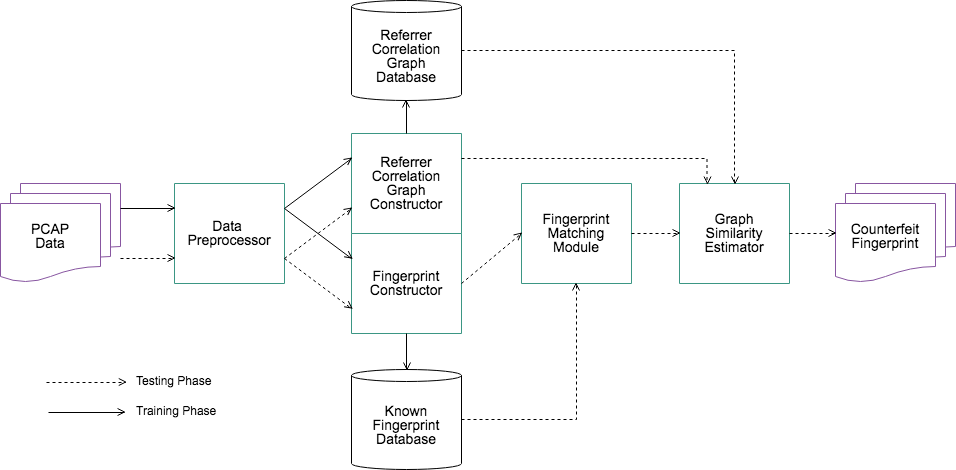
\includegraphics[width=400pt]{image/sa.png}
\caption{An overview of our counterfeit fingerprint detection system. Five subsystems are depicted: (1) data preprocessor subsystem, (2) fingerprint constructor subsystem, (3) fingerprint matching subsystem, (4) referrer correlation graph constructor subsystem, and (5) graph similarity estimator subsystem. The system only takes the PCAP files of outbound HTTP traffics as input. In training phase, subsystem (1) and (2) passively extract the benign fingerprint from an application's outbound HTTP traffic, and subsystem (3) could use fingerprints to classify benign traffic in the testing phase. We note that referrer correlation extraction in the subsystem (4) is a key step, in the sense that if it can extract discriminative features for counterfeit fingerprint detection, the detection in the subsystem (5) is relatively straightforward.}
\label{fig:sa}
\end{figure*}

\subsection{Browser Traffic Extractor}

For most cases of client-side attacking, hackers whose general goal is to steal valuable data before malware connects to C\&C server. As a result, PCAP files, that contain specific network characteristics of an application (e.g., browser) for each host in the enterprise. 

%To generate fingerprint for each browser, our approach first extracts various entities from PCAP files. Table~\ref{tbl:log_01} shows 6 heterogeneous fields which can be extracted from each one-line log, including domain ({\em Domain}), destination IP ({\em DstIP}), user-agent ({\em User-agent}), accept language ({\em Accept-Lang}), length ({\em Len}), and constant field ({\em Constant}). The reason for choosing these 6 fields for browser traffic classification can be summarized as followings and fingerprint construction is represented in next subsection. 

%\begin{table}[]
%\centering
%\caption{Fields and Values of Database in a PCAP File}
%\label{tbl:log_01}
%\begin{tabular}{ll}
%\hline\hline
%Field                           & Value for Instance                                               \\\hline
%{\em Domain}            & yahoo.com.tw                                                      \\
%{\em DstIP}                & 140.92.88.140                                                     \\
%{\em User-agent}      & Mozilla/5.0 (Windows NT 6.1; Win64; x64) ...  \\
%{\em Accept-Lang}   & zh-TW                                                                  \\
%{\em Len}                   & 1253                                                                     \\
%{\em Constant}          & If-Modified-Since, Cookie, Connection, ...       \\\hline\hline
%\end{tabular}
%\end{table}

To generate fingerprint for each browser, our approach first extracts various entities from PCAP files. Table~\ref{tbl:log_01} shows 4 heterogeneous fields which can be extracted from each one-line log, including domain ({\em Domain}), user-agent ({\em User-agent}), accept language ({\em Accept-Lang}), and referrer ({\em Referrer}). The reason for choosing these 4 fields for browser traffic classification can be summarized as followings and fingerprint construction is represented in next subsection. 

\begin{table}[]
\centering
\caption{Fields and Values of Database in a PCAP File}
\label{tbl:log_01}
\begin{tabular}{ll}
\hline\hline
Field                           & Value for Instance                                               \\\hline
{\em Domain}            & www.yongchang-yc.com.tw                              \\
{\em User-agent}      & Mozilla/5.0 (Windows NT 6.1; Win64; x64) ...  \\
{\em Accept-Lang}   & zh-TW,zh;q=0.9,en-US;q=0.8,en;q=0.7          \\
{\em Referrer}           & www.yongchang-yc.com.tw                               \\\hline\hline
\end{tabular}
\end{table}

In previous research \cite{bortolameotti2017decanter}, Bortolameotti et al. identified two types of HTTP applications (e.g., $browser$ and $background$). This subsection aims to filter logs of a PCAP file according to the {\em User-agent}, because we focus on counterfeit fingerprints of browser network activities. To identify browser activities, the browser flags we defined are "Mozilla", "Opera", "MQQBrowser", "UCWEB",  "NOKIA5700", "Openwave", "Safari", and "Chrome", and which are used for string matching in field {\em User-agent}. Furthermore, in the testing phase, an implementation time-slot $t$ is a fixed time window of $T$ minutes, and the filtered logs is passed to the next module after $t$ ends.

%Furthermore, in both training and testing phase, a filtered logs is continuously passed to the next module in the real time.

\subsection{Fingerprint Constructor}

Single feature (e.g., {\em User-agent}) isn't effective enough to filter normal network activities \cite{bortolameotti2017decanter} \cite{kheir2013analyzing}. Therefore, we consider multiple features such as {\em User-agent} and {\em Accept-Lang} for fingerprint generation, and {\em Domain} and {\em Referrer} would be used for constructing the correlation graph in other subsection. In our assumption, hacker can't be so lucky to guess all parameters of {\em User-agent} and {\em Accept-Lang} at the same time. In this subsection, we denote a set of {\em User-agent} $U = \begin{Bmatrix} u_{1}, & ... & , u_{n} \end{Bmatrix}$, and a set of {\em Accept-Lang} $L = \begin{Bmatrix} l_{1}, & ... & , l_{m} \end{Bmatrix}$ where $\left | U \right | = n$ and $\left | L  \right | = m$. Furthermore, our approach makes fingerprint $f = (u_{i}, l_{j})$ where $i = 1 \sim n$, $j = 1 \sim m$, and $\left | f \right | = n \times m $. Matching testing browser fingerprint to knowns which is trained and stored in database, and we would briefly show the similarity estimation in following module.

\subsection{Fingerprint Matching Module}

Matching fingerprint we used is an easy comparison in this module \cite{bortolameotti2017decanter}. In training phase, we take fingerprints $f_{b_{i}}$ for each browser $b_{i}$. If our approach constantly runs in testing mode, we must obtain other browser $b_{j}$ fingerprints $f_{b_{j}}$. Then, we use edit distance to estimate fingerprint matching result $d(f_{b_{i}}, f_{b_{j}}) $ which is shown as in Equation ~\ref{eq:edit}.

\begin{equation}
        \label{eq:edit}
        d(f_{b_{i}}, f_{b_{j}}) = \sum_k \left |  f_{b_{i_{k}}} - f_{b_{j_{k}}} \right |  
\end{equation}

\subsection{Referrer Correlation Graph Constructor}

A call graph models a connection between URLs as a directed graph whose vertices, representing the domain name is interconnected through directed edges which have reference correlation. According to fields {\em Domain} and {\em Referrer}, a vertex could be represented as domain name which is extracted from a URL of the field, and an directed edge shows the reference correlation from {\em Referrer} to {\em Domain}. The example directed graph is depicted in figure \ref{fig:ref_graph}. According to \cite{kinable2011malware}, call graphs are formally defined as a directed graph $G$ with vertex $V = V(G)$, representing the domain name, and edge $E = E(G)$, where $E(G) \subseteq V(G) \times V(G) $, in correspondence with the reference correlation.

\begin{figure}[!t]
\centering
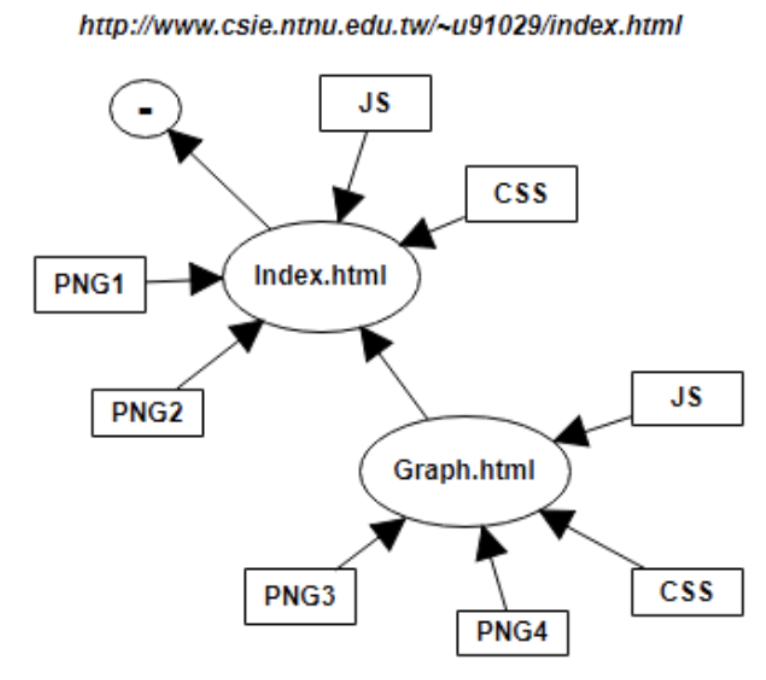
\includegraphics[width=250pt]{image/ref_graph.png}
\caption{An Example of a referrer correlation graph generated from a browser traffic. The ellipse nodes represent the webpage that users have viewed by clicking the hyperlink in the browser. The rectangular nodes represent the sources that the web page needed. The arrow pointing means which node is referred by the web page.}
\label{fig:ref_graph}
\end{figure}

A candidate set $S = \{st_1, st_2, ..., st_{ns}\}$ that contains all domain names filtered by fingerprint matching module and derived from $D_i$. Note that $ns$ is the total number of derived domain names in $D_i$. Given the dataset $D_i$ containing $i^{th}$ domain name; $i=1,...,ns$, and its referrer correlation based on the dataset should includes an $1 \times ns$ adjacency vector ($ADJ$), as following:

\begin{equation*}
\begin{split}
ADJ(i) = 
\left[
\begin{array}{ccccc}
tp_{i,1} & \ldots & tp_{i,j} & \ldots & tp_{i,ns}\\
\end{array}
\right]
\end{split}
\end{equation*}

where for each $i$ and $j$, $tp_{i,j}$ represents a directed edge which is referrer correlation from $j^{th}$ domain name to $i^{th}$ candidate domain.

\begin{equation*}
\begin{array}{ll}
\forall\mbox{ }i,j=1,...,ns, &\\ 
tp_{i,j} = \mbox{\#connections from }\mbox{$st_j$}\mbox{ to }\mbox{$st_i$}\mbox{ in }\mbox{$D_i$}			 
\end{array}
\end{equation*}

\subsection{Graph Similarity Estimator}

Our proposed approach relies on appropriate estimating deviation from domain name's new referrer correlation to its benign one. In this paper, domain name's referrer correlation is summarized as patterns represented by adjacency vector, as a result, deviation measuring can be realized by using graph edit distance (GED) to quantify similarity (or dissimilarity) between different vectors.   
The formal graph edit distance between two graphs $G_{1}$ and $G_{2}$, written as $GED(G_{1},G_{2})$ can be defined as following:

\begin{equation}
GED(G_{1},G_{2}) = \min\limits_{(e_{1},...,e_{k}) \in P(G_{1}, G_{2})}\sum\limits_{i=1}^{k}cost(e_{i}),
\label{equ:ged_idea}
\end{equation} 

where $P(G_{1}, G_{2})$ denotes the universal set of editing paths isomorphically transforming $G_{1}$ into $G_{2}$, and $cost(e_{i})$ is the cost of each graph editing operation, $e_{i}$.

With respect to referrer correlation graph in our method, calculation of GED on two graphs can then be implemented by following equation (\ref{equ:ged_implementation}): 

\begin{equation}
GED(ADJ(a), ADJ(b)) = \sum\limits_{j=1}^{ns}\left|tp_{a,j} - tp_{b,j}\right|,
\label{equ:ged_implementation}
\end{equation}

where $ADJ(a)$ and $ADJ(b)$ are adjacency vectors of two referrer correlation graphs, as well as $tp_{a,j}$ and $tp_{b,j}$ are the corresponding references in $ADJ(a)$ and $ADJ(b)$, respectively. The $ns$ is the number of candidate domain names after fingerprint matching.